\section{Experiments and Results}
\label{sec:experiments}

\subsection{Full-Rate (60~Hz) Intent Bandwidth and Action Diagnostics (Task~1)}
\label{sec:exp_m1}
PCA on 1.23M deterministic transitions from the frozen Task~1 reference expert ($P_E = 26.11$) reveals a flat action spectrum: $k=2/4/8$ components capture only $35.8\% / 56.8\% / 81.1\%$ of 20-D action variance, and 95\% requires 14 components (vs.\ 2~PCs for $>80\%$ in static human grasping \citep{santello1998postural}).
Commands are near bang-bang (62.2\% of entries at $\pm 1$, 20--32\% step-to-step sign flips), and joint-position PCA confirms that this high dimensionality is intrinsic rather than a bang-bang artifact (Appendix~\ref{app:stage1}).

Table~\ref{tab:m1_60hz} reports 60~Hz goal-hidden recovery across interfaces ($n=3$ seeds; $n=5$ for \texttt{goal-4}).
Without intent, \texttt{blind} collapses ($P_{\mathrm{blind}} = 0.006$), and scalar distance (\texttt{obj-1}) provides no directional cue.
Action recovery climbs monotonically with $k$ and saturates at \textbf{\texttt{hand-8}} (\textbf{86.6\%}, Bonferroni-significant vs.\ \texttt{blind}, $p=0.006$), matching full-rank \texttt{hand-20} (80.5\%) and 4-D \texttt{goal-4} (78.0\%), while outperforming \texttt{obj-4} (32.8\%) and \texttt{wrist-2} (29.2\%).
Separating wrist and finger PCA (\texttt{wrist2-finger-2/6}: 55.0\% / 65.3\%) retains less total action variance and does not improve over joint whole-hand PCA ($p=0.16$; Table~\ref{tab:app_pca}, Appendix~\ref{app:stats}).

\begin{table}[t]
  \centering
  \caption{Task~1 (goal-hidden, 60~Hz) performance recovery ($P_E=26.11$, $P_{\mathrm{blind}}=0.006$; $n=3$ seeds except \texttt{goal-4} with $n=5$). At full rate, \texttt{hand-8} saturates action recovery and matches \texttt{goal-4}.}
  \label{tab:m1_60hz}
  \small
  \begin{tabular}{lcccc}
    \toprule
    Intent Interface & Dim $k$ & Recovery (Final) & AUC & Seeds $\ge 0.8 P_E$ \\
    \midrule
    \texttt{blind} (lower bound) & 0 & $0.000 \pm 0.000$ & $0.000$ & 0/3 \\
    \texttt{obj-1} & 1 & $0.001 \pm 0.001$ & $0.000$ & 0/3 \\
    \texttt{wrist-2} & 2 & $0.292 \pm 0.250$ & $0.154 \pm 0.141$ & 0/3 \\
    \texttt{obj-4} ($\Delta\theta=0.5$~rad) & 4 & $0.328 \pm 0.116$ & $0.110 \pm 0.047$ & 0/3 \\
    \texttt{hand-2} & 2 & $0.504 \pm 0.079$ & $0.367 \pm 0.084$ & 0/3 \\
    \texttt{hand-4} & 4 & $0.714 \pm 0.213$ & $0.510 \pm 0.165$ & 1/3 \\
    \texttt{goal-4} (rate grid, $n=5$) & 4 & $0.780$ & --- & --- \\
    \texttt{hand-20} & 20 & $0.805 \pm 0.017$ & $0.574 \pm 0.023$ & 2/3 \\
    \textbf{\texttt{hand-8}} & 8 & $\mathbf{0.866 \pm 0.112}$ & $\mathbf{0.623 \pm 0.073}$ & 2/3 \\
    \bottomrule
  \end{tabular}
\end{table}

\subsection{Rate Reversal, Channel Degradation, and Staleness (Task~1)}
\label{sec:exp_rate}
\paragraph{Rate reversal and Slow-Expert control.}
Under zero-order hold refresh ($N \in \{1, 6, 12, 30\} \leftrightarrow 60/10/5/2$~Hz), the 60~Hz ranking reverses sharply (Figure~\ref{fig:channel_degradation}a).
Across $n=5$ seeds, \texttt{hand-8} and \texttt{goal-4} match at 60~Hz (80\% vs.\ 78\%, Welch $p=0.86$), but at 10~Hz \texttt{hand-8} plunges to \textbf{19\%} while \texttt{goal-4} retains \textbf{71\%} ($p=0.0003$; persisting after resuming \texttt{hand-8} to 10,000 iterations at 22\%, and dropping to 3\% with 62\% cube drops under eval-only hold; Appendix~\ref{app:stats}).
At 5~Hz and 2~Hz, \texttt{goal-4} retains \textbf{65\%} and \textbf{44\%}, whereas \texttt{hand-8} collapses to 10\% and \textbf{2.5\%} ($p<0.0001$), \texttt{obj-4} to 13\% and 2\%, and \texttt{hand-2} to 0\%.
In the \textbf{Slow Expert} control (goal visible, 20-D motor actions held for $N$ steps), $P/P_E$ drops from 97\% (60~Hz) to \textbf{11.8\% $\pm$ 3.8\%} at 10~Hz ($\approx 15\%$ at 10,000 iterations), \textbf{0.1\%} at 5~Hz, and \textbf{0.0\%} at 2~Hz—never exceeding 10~Hz \texttt{hand-8} ($p \ge 0.33$) and far below \texttt{goal-4} ($p \le 0.001$).

\paragraph{Staleness mechanism, latency law, and quantization.}
Offline rollout analysis shows that performance across all interfaces collapses onto a single monotonic curve when plotted against \emph{inter-update staleness} relative to task tolerance (Figure~\ref{fig:app_staleness}, Appendix~\ref{app:stats}): held \texttt{hand-$k$} captures only $\sim 5\%$ of action variance at 20~Hz and performs worse than the mean action at $\le 10$~Hz; moving \texttt{obj-4} waypoints drift $>0.1$~rad stale on 81\% of steps at 2~Hz (vs.\ 26\% for \texttt{goal-4} on the same trajectory); whereas \texttt{goal-4} changes only upon goal completion (every 21.9 steps on average).
Latency and quantization confirm this mechanism (Figure~\ref{fig:channel_degradation}b):
at $d=6$ steps (0.1~s eval-only delay), \texttt{hand-8} collapses to \textbf{0.3\%} (91--97\% drops), while \texttt{goal-4} degrades smoothly across 0 / 0.1 / 0.5 / 1.0 / 2.0~s (77\% / 64\% / 39\% / 26\% / 16\%), matching Eq.~\ref{eq:waiting} within \textbf{0.007} recovery per seed (training under $d \ge 30$ yields slower controllers below the line; Appendix~\ref{app:stats}).
Under scalar quantization, \texttt{goal-4} is lossless at 8~bits/component (32~bits/goal, 77\%) but drops to 12\% at 4~bits and 1\% at 3~bits as rounding error approaches the 0.1~rad tolerance.

\begin{figure}[t]
  \centering
  \begin{subfigure}[b]{0.38\linewidth}
    \centering
    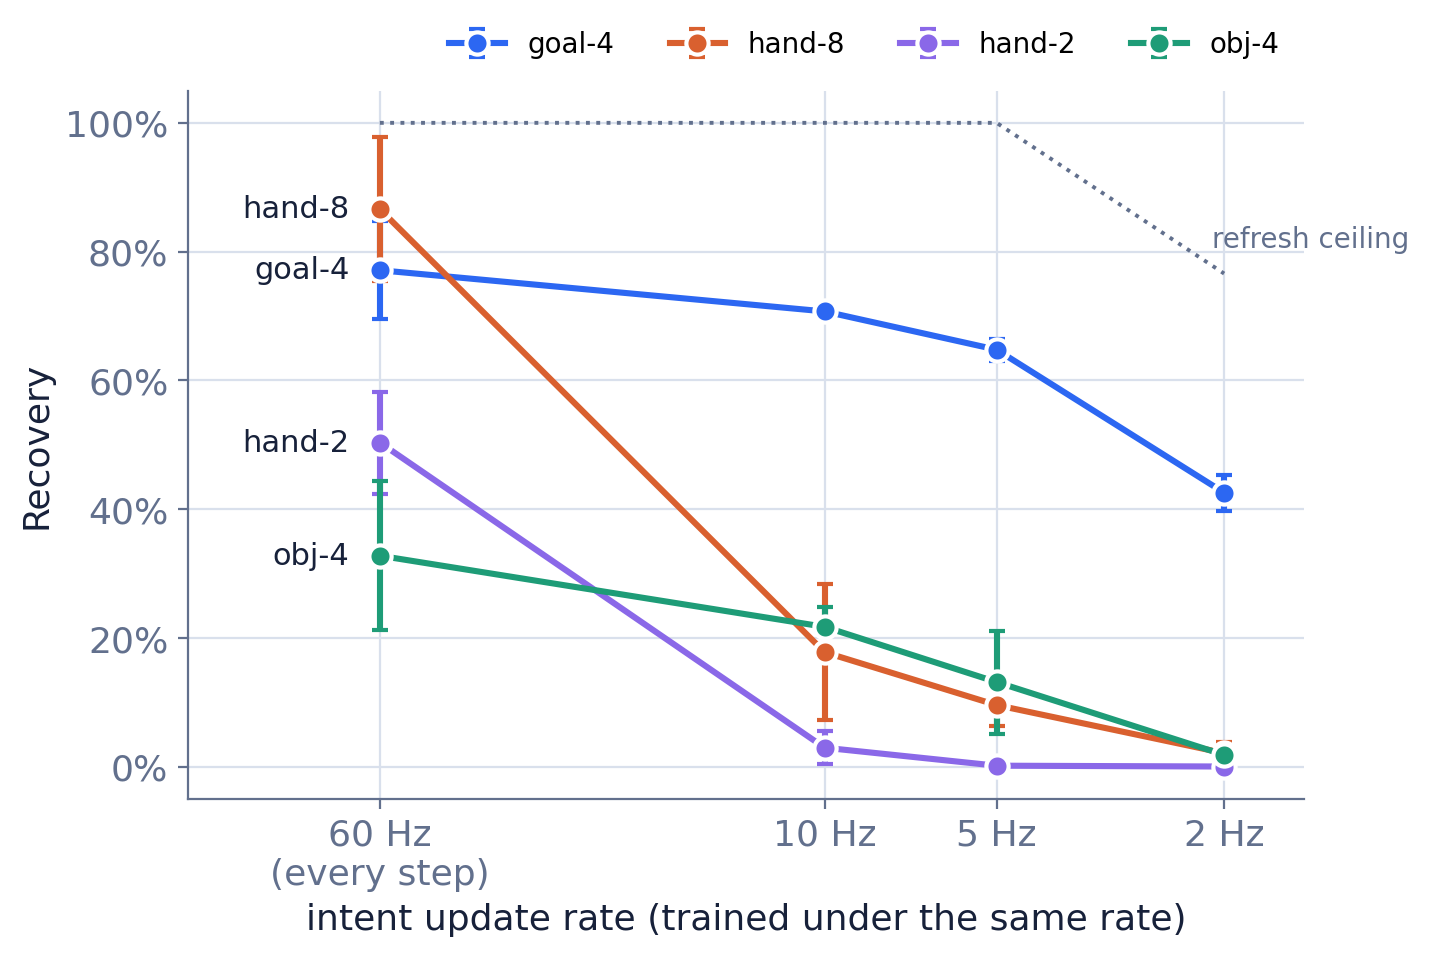
\includegraphics[width=\linewidth]{figures/rate_sweep.png}
    \caption{Rate sweep (trained under hold)}
  \end{subfigure}\hfill
  \begin{subfigure}[b]{0.60\linewidth}
    \centering
    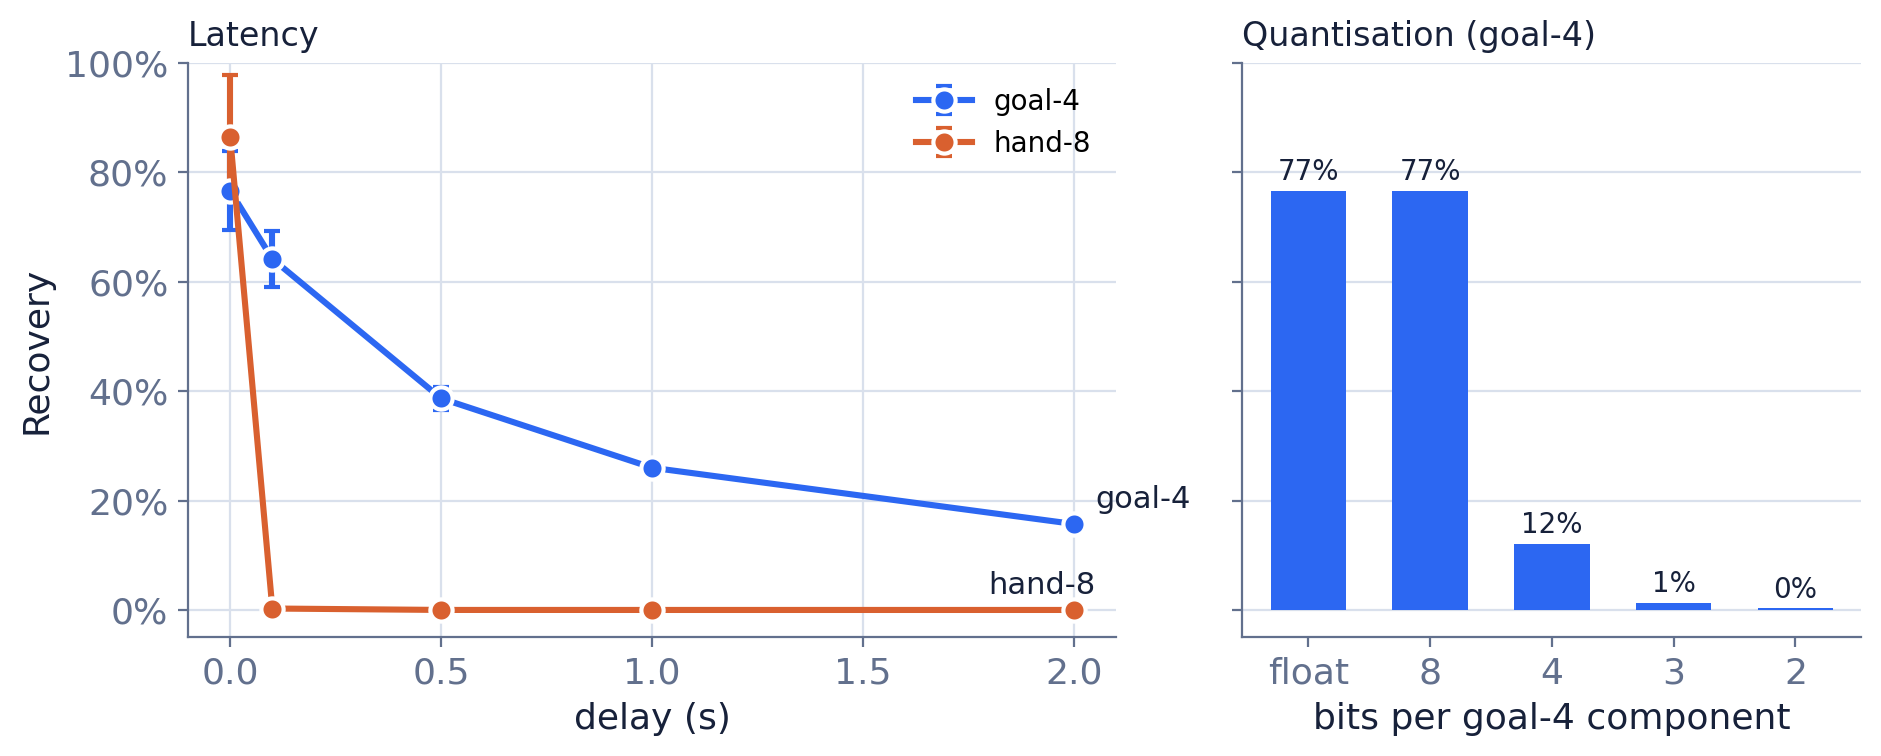
\includegraphics[width=\linewidth]{figures/channel_delay_bits.png}
    \caption{Eval-only latency and scalar quantization}
  \end{subfigure}
  \caption{Channel degradation on Task~1. (a)~Rate reversal between \texttt{goal-4} and \texttt{hand-8} across 60--2~Hz. (b)~Under latency, \texttt{hand-8} fails at 0.1~s while \texttt{goal-4} tracks Eq.~\ref{eq:waiting}; quantization requires $\ge 8$~bits/component (staleness collapse in Appendix~\ref{app:stats}).}
  \label{fig:channel_degradation}
\end{figure}

\subsection{Cross-Task Generalization and the ``Stale Goal'' Trap (Task~2: $z$-Axis)}
\label{sec:exp_m2}
On Task~2 ($P_E = 31.14$), the goal-hidden \texttt{blind} policy already reaches $P_{\mathrm{blind}} = 19.66$ (63\% of $P_E$) by exploiting a goal-free unidirectional spinning heuristic (Appendix~\ref{app:stats}).
Even so, the rate reversal replicates cleanly: at 60~Hz, \texttt{hand-8} (36.7), \texttt{hand-4} (40.1), \texttt{goal-yaw} (35.7), and \texttt{goal-4} (32.7) perform comparably ($p \ge 0.23$).
At 10~Hz, our pre-registered $n=5$ seed test confirms that task-native \texttt{goal-yaw} ($31.05 \pm 2.38$, \textbf{99.2\%} recovery) significantly outperforms \texttt{hand-8} ($23.06 \pm 4.50$, \textbf{29.6\%} recovery; Welch $p=0.0124$, Mann--Whitney $U=0, p=0.0079$).
Crucially, at 2~Hz both \texttt{goal-yaw} (16.2) and \texttt{hand-8} (11.7) fall \emph{below} \texttt{blind} (19.7; $p=0.03$ for \texttt{hand-8}), exposing a \textbf{stale-goal trap} where chasing outdated goals underperforms a goal-free heuristic.

\subsection{Multi-Skill Hinged Cube and Boundary Conditions (Task~3)}
\label{sec:exp_task3}
Table~\ref{tab:unified_v4} compares multi-skill controllers on the hinged cube.
Raw two-expert switching suffers 14--26\% handoff drops and 14--19\% turn stalls; fine-tuning the turn expert on Stage~1 \texttt{up} end states cuts drops to 1--2\% and lifts \texttt{up,turn} to 7.51 cycles/600 steps.
Resolving the v1--v3 exploits (Appendix~\ref{app:unified_debug}), \textbf{\texttt{Unified v4}} reaches \textbf{18.02} \texttt{up,turn} cycles (2 seeds: 18.88 / 17.16; $2.4\times$ tuned handoff) and 10.08 \texttt{any,up,turn} cycles with $<0.02\%$ stalls and balanced $\pm 90^\circ$ turns.

\begin{table}[t]
  \centering
  \caption{Task~3 multi-skill composition (per 600 steps, 1,024 envs). \texttt{Unified v4} (2-seed mean: 18.88 / 17.16) outperforms handoff-tuned switching by $2.4\times$ with near-zero stalls.}
  \label{tab:unified_v4}
  \footnotesize
  \setlength{\tabcolsep}{4pt}
  \begin{tabular*}{\linewidth}{@{\extracolsep{\fill}}lccccc}
    \toprule
    Controller & \texttt{up,turn} & \texttt{any,up,turn} & Stalls ($>120$) & Falls (\texttt{up,turn}) & Turn Steps (med.) \\
    \midrule
    Two-Expert (raw) & 4.61 & 3.50 & 14--19\% & 0.70 & 33--35 \\
    Two-Expert (tuned) & 7.51 & 5.48 & 3.5--4.5\% & 0.10 & 33 \\
    \textbf{\texttt{Unified v4} (2-seed mean)} & \textbf{18.02} & \textbf{10.08} & \textbf{0.02\%} & \textbf{0.013} & \textbf{18--19} \\
    \bottomrule
  \end{tabular*}
\end{table}

Multi-skill switching reproduces both Part~I laws: two-expert selector hold/delay (E2') tracks $600/(T_0+L\cdot w)$ without added drops (Appendix~\ref{app:stats}), and goal-hidden students on \texttt{Unified v4} (E3, $n=3$) reproduce the 10~Hz reversal on \texttt{up,turn} (60~Hz: \texttt{hand-8} 9.68 vs.\ \texttt{goal-7} 6.20; 10~Hz: \texttt{goal-7} retains \textbf{69\%} [4.30] vs.\ \texttt{hand-8} \textbf{4\%} [0.36], $p=0.063$; mixed-phase \texttt{any}/\texttt{goal-11} diagnostics in Appendix~\ref{app:stats}).
By contrast, an 8-seed study on isolated 1-DOF face turns (E1) reveals a \textbf{boundary condition}: take-off ($>10$ turns) is bimodal and seed-driven (4/16 for both \texttt{goal-yaw} and \texttt{hand-8}, Fisher $p=1.0$), and taken-off \texttt{hand-8} runs reach expert level even at 10~Hz (23.2--34.0 turns) despite negative action-reconstruction variance ($-7\%$).
An offline MLP probe resolves this paradox: on 1-DOF face turns, held \texttt{hand-8} at 10~Hz still retains \textbf{53\%} of hidden goal-error variance ($R^2=0.53$, vs.\ only \textbf{22\%} on 3D Task~1), effectively degenerating into a goal code (before still collapsing at 2~Hz to 13\% vs.\ 60--82\% for \texttt{goal-yaw}).

\subsection{End-to-End Visual VLM Control over Frozen \texttt{Unified v4} (Scheme~C)}
\label{sec:exp_vlm}
\paragraph{Execution ceiling and zero-shot bottlenecks.}
Wrapping frozen \texttt{Unified v4} in our 96-state external-goal interface (P2.1) yields \textbf{100.0\%} closed- and open-loop BFS execution (2,048/2,048 episodes, 0.0\% drops, 0.0\% hinge drift $>45^\circ$, 16.5 steps/macro-action) and \textbf{0.0\%} drops over 4.0~s (240-step) holds—a zero-loss physical floor ($P_{\mathrm{Oracle}}=1.000$).
On this floor, zero-shot \texttt{Qwen3-VL-8B-Instruct} (pipeline verified on EmbSpatial 78.24\% vs.\ 78.5\% official, Appendix~\ref{app:scheme_c}) exhibits two bottlenecks:
(1)~\emph{Spatial grounding}: on 180 held-out test frames (CircularEval), 3-view \texttt{montage} reaches 90.0\% on coarse \texttt{up} color but only \textbf{7.5\%} on narrow-band \texttt{band} (0.0\% all-levels), whereas adding Set-of-Mark \texttt{[1]/[2]} jumps \texttt{turned} to 80.0\% and \texttt{band} to 67.9\% (50.9\% all-levels);
(2)~\emph{Relational planning}: given oracle \texttt{relational} text state, zero-shot greedy success falls across $L=1..4$ (100\% / 56\% / 14\% / 4\%, overall 43.5\%), while Pass@8 stays at 74\%/66\%/54\%.

\paragraph{Perception generalization, overfitting audit, and forgetting check.}
Full held-out perception, benchmark, and closed-loop generalization tables appear in Appendix~\ref{app:scheme_c} (Tables~\ref{tab:vlm_perception}--\ref{tab:app_cl_gen}).
Frozen-ViT Map-then-Reason LoRA SFT (\texttt{C1-v1}, 0.51\% trainable parameters, zero SoM tags) lifts canonical \texttt{band} accuracy from 7.5\% to \textbf{99.4\%} (99.4\% \texttt{@nohand}) and generalizes strongly to swapped colors (OOD G$\leftrightarrow$B \textbf{96.2\%}), novel palettes (89.9\% \texttt{band}), and two unseen cameras (\texttt{s130+top} \textbf{83.3\%}), while preserving EmbSpatial ($-1.89\%$), MMStar ($-1.13\%$), and BLINK ($-3.84\%$).
Auditing \texttt{C1-v1} exposes format/abstention overfitting on unseen inverse prompts (\texttt{v3}: 36.8\%) and unanswerable frames (CBD: 0.0\%); our data-centric \textbf{\texttt{C1-v2}} (1 epoch, multi-template + CBD + 30\% augmentation + cyclic $\mathbb{Z}_4$ CoT) maintains 98.7\% canonical and 96.2\% OOD accuracy while lifting CBD abstention to \textbf{100.0\% (21/21)} (0.6\% false-CBD), unseen \texttt{v3} to \textbf{59.2\%} (\texttt{turned} 96.7\%), and open-loop \texttt{turn} optimality from 77.1\% to \textbf{89.6\%}.

\paragraph{Closed-loop manipulation, GRPO saturation, and real 60~Hz Isaac Lab verification.}
Table~\ref{tab:vlm_closedloop} summarizes multi-turn closed-loop control across all 96 states.
On the 200-task image pool, \texttt{C1-v1} reaches \textbf{100.0\% (181/181)} at 1.216$\times$ rounds with zero illegal actions because closed-loop visual feedback self-corrects occasional $\pm 90^\circ$ sign flips; consequently, outcome-reward GRPO (\texttt{C2}) hits DAPO zero-variance saturation (74--82\% all-pass groups), whereas explicit cyclic CoT in \texttt{C1-v2} cuts the rounds ratio to \textbf{1.121$\times$}.
Deploying \texttt{C1-v1} in \textbf{real 60~Hz Isaac Lab online 3-camera rendering} over 128 physical episodes ($L=1..4$, 32/level, 368 rounds) achieves \textbf{100.0\% (128/128)} success, \textbf{0.0\% falls}, \textbf{98.9\%} live 96-state accuracy, \textbf{1.175$\times$} rounds ratio, and \textbf{15.7 steps (0.26~s)} per macro-action—matching the BFS Oracle with zero sim-to-offline gap.

\begin{table}[t]
  \centering
  \caption{Multi-turn closed-loop manipulation over frozen \texttt{Unified v4} (offline 200-task image pool and real 60~Hz Isaac Lab online 3-camera physics).}
  \label{tab:vlm_closedloop}
  \footnotesize
  \setlength{\tabcolsep}{3.5pt}
  \begin{tabular*}{\linewidth}{@{\extracolsep{\fill}}lcccccc}
    \toprule
    Method / Eval Env & Eps & Success & Falls & Rounds/$L^*$ & State Acc & Illegal \\
    \midrule
    Zero-Shot Text (Oracle) & 200 & 43.5\% & --- & --- & (Oracle text) & --- \\
    BFS Oracle (Isaac Lab \texttt{v4}) & 2,048 & \textbf{100.0\%} & 0.0\% & 1.000$\times$ & (Oracle sim) & 0.0\% \\
    \midrule
    \texttt{C1-v1} (200-Task Pool) & 181 & \textbf{100.0\%} & --- & 1.216$\times$ & 91.7\% & 0.0\% \\
    \texttt{C2} GRPO (Gnd./Term., Pool) & 182 / 181 & \textbf{100.0\%} & --- & 1.236 / 1.216$\times$ & 90.2 / 91.5\% & 0.0\% \\
    \texttt{C1-v2} (200-Task Pool) & 181 & 98.9\% & --- & \textbf{1.121$\times$} & 90.5\% & 0.4\% \\
    \textbf{\texttt{C1-v1} (Isaac Lab Online)} & \textbf{128} & \textbf{100.0\%} & \textbf{0.0\%} & \textbf{1.175$\times$} & \textbf{98.9\%} & \textbf{0.0\%} \\
    \bottomrule
  \end{tabular*}
\end{table}
